Kliknięcie prawym przyciskiem myszy na ikonie programu w lasku launchera daje dostęp do SzybkiejListy (QuickList) z dodatkowymi opcjami oferowanymi przez ten program. Przykłądowo lista dla pakietu biurowego LibreOffice zawiera skróty do bezpośredniego otworzenia procesora tekstu Writer, akrusza kalkulacyjnego Calc, prezentacji impress i innych.

Dzięki programowi QuickList Editor możliwe jest zarzadzanie zawartością SzybkichList --- dodwanie nowych opcji, usówanie starych i modyfikowanie istniejących. Aby zainstalować QLE uruchom \menu{{Oprogramowanie i Aktualizacje}>{Inne oprogramowanie}>{Dodaj\ldots}}. W pole \textcolor{ubuntu_orange}{Wiersz APT} wpisz:
\begin{lstlisting}
http://ppa.launchpad.net/vlijm/qle/ubuntu
\end{lstlisting}
Kliknij na przycisk \textcolor{ubuntu_orange}{Dodaj Zasób} i potwierdź swoim hasłem. Kiedy spróbujesz wyjść z tego programu zostaniesz poinformowany o potrzebie uaktualnienia listy pakietów. Zrób to i poczekaj chwilę. Kiedy operacja zostanie zakończona otwórz terminal i zainstaluj program qle:
\begin{lstlisting}[language=bash]
sudo apt-get install qle
\end{lstlisting}
\begin{itemize}
\item \textcolor{ubuntu_orange}{sudo} --- wykonuje dalsze polecenia z uprawieniami administratora systemu.
\item \textcolor{ubuntu_orange}{apt-get} --- program do zarządzania zainstalowanym oprogramowaniem.
\item \textcolor{ubuntu_orange}{install} --- informujesz apt, że chcesz zainstalować paczkę z oprogramowaniem.
\item \textcolor{ubuntu_orange}{qle} --- nazwa paczki do zainstalowania.
\end{itemize}
\begin{center}
	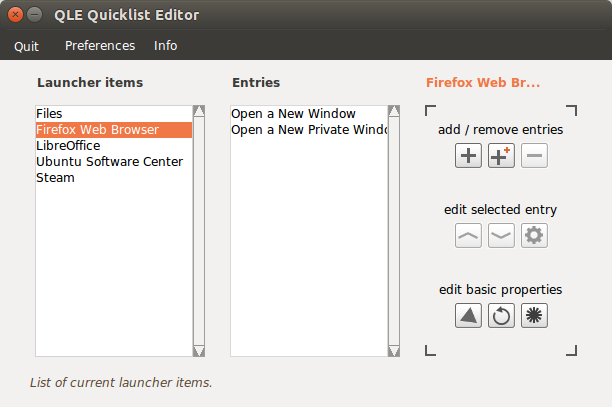
\includegraphics[width=\linewidth]{images/programy_qle.png}
\end{center}

Aby uruchomić ten program w Dashu wpisz \textcolor{ubuntu_orange}{QLE}